\section{Payload Design and Operation}
\label{sec:Hardware}

\begin{figure}[!ht]
\begin{center}
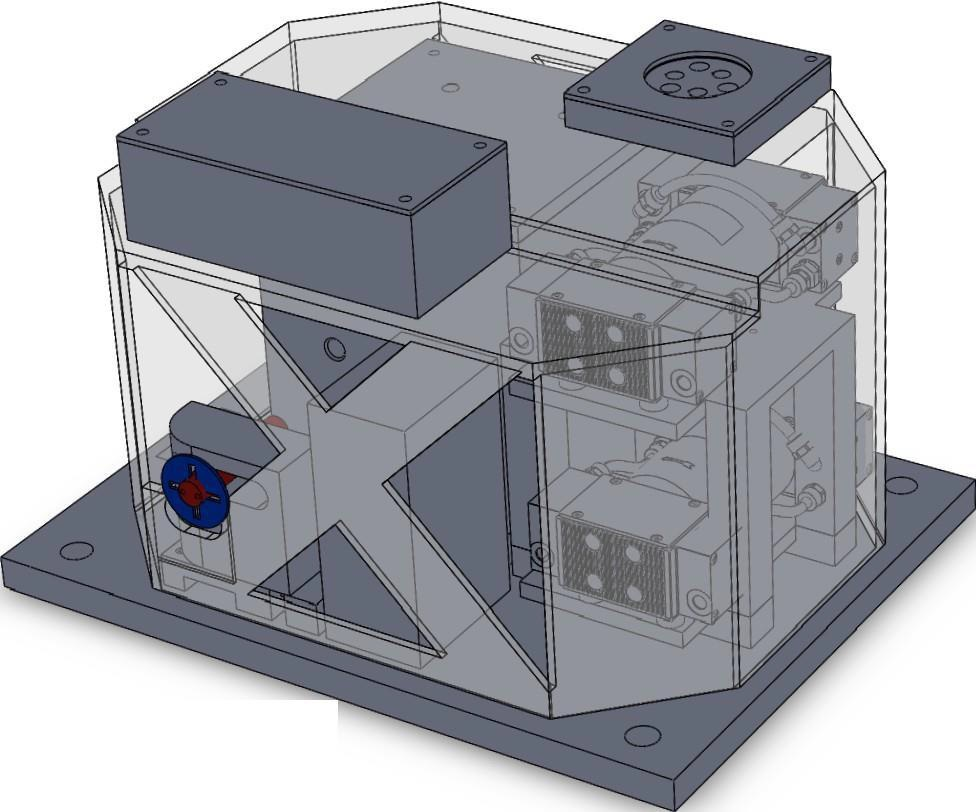
\includegraphics[width=.75\textwidth]{./Figures/payload_1.jpg}
\caption{Solidworks design of the SORA payload.}
\label{fig:payload} 
\end{center}
\end{figure}

The SORA 2.0 payload will have an upgrade and more efficient flight computer, a fully developed astrobiology system and a MiniPIX USB silicion detector.  The astrobiology system will build upon the previous mission, but this time we are seeking to capture and culture any microorganisms we may find.  Our previous mission in 2017 confirmed that our astrobiology system functions well beyond expectations and that there are microorganisms in the upper atmosphere.

\begin{figure}[!ht]
\begin{center}
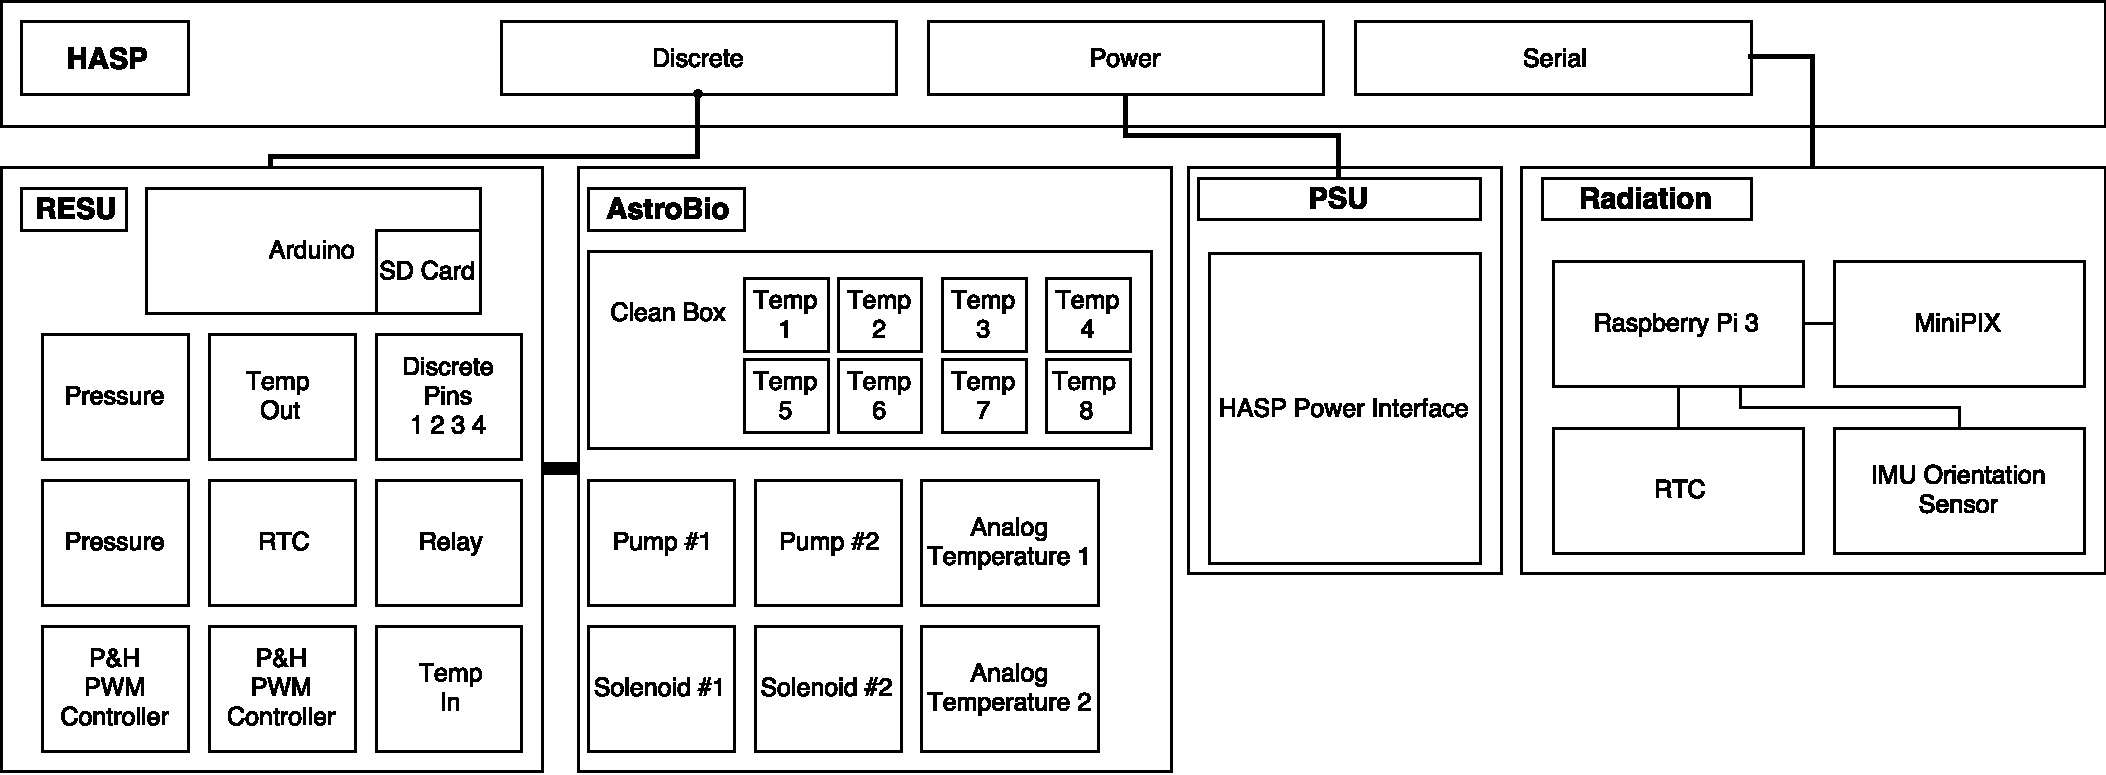
\includegraphics[width=.75\textwidth]{./Figures/RESU_2018.pdf}
\caption{Solidworks design of the SORA payload.}
\label{fig:payload} 
\end{center}
\end{figure}
